\documentclass[12pt]{b-thesis}
\usepackage{tabularx}
\usepackage{color}
\usepackage{url}
\usepackage[dvipdfmx]{graphicx}
\usepackage{comment}
\usepackage{amsmath}
\usepackage{ascmac}
\usepackage{amsthm}
\usepackage{amssymb}
\usepackage{otf}
\usepackage{url}

\usepackage{threeparttable}
\newcommand{\bhline}[1]{\noalign{\hrule height #1}}

%%%%%%%%%%%% FOR listing %%%%%%%%%%%%%%%%%%%%

\usepackage{listings}
\definecolor{hellgelb}{rgb}{1,1,0.8}
\definecolor{colKeys}{rgb}{0,0,1}
\definecolor{colIdentifier}{rgb}{0,0,0}
\definecolor{colComments}{rgb}{1,0,0}
\definecolor{colString}{rgb}{0,0.5,0}
\def\lstlistingname{ソースコード}
\renewcommand{\thelstnumber}{\arabic{lstnumber}:}

\lstset{
    float=hbp,
    basicstyle=\ttfamily\small,
    identifierstyle=\color{colIdentifier},
    keywordstyle={\color[rgb]{0,0,0.7}},
    stringstyle={\color[rgb]{0.8,0.2,0}},
    commentstyle={\color[rgb]{0,0.4,0}},
    columns=fixed,
    tabsize=2,
    frame=single,
    framexleftmargin=8mm,
    xleftmargin=8mm,
    numbersep=1zw,
    extendedchars=true,
    showspaces=false,
    showstringspaces=false,
    numbers=left,
    breaklines=true,
    backgroundcolor=\color{white},
    breakautoindent=true,
    captionpos=b,
    language=bash
}

%%%%%%%%%%%% FOR listing ここまで%%%%%%%%%%%%%%

%PDFファイルの栞日本語化
\AtBeginDvi{\special{pdf:tounicode 90ms-RKSJ-UCS2}}

\begin{document}
%%%%%    Title    %%%%%
\typeout{Titlepage}
\title{ランダムウォークによるグラフ取得における\\ノード ID 再配置手法}
\titleinenglish{}
\teacher{金子 晋丈 准教授}
\subteacher{}
\course{情報工学}
\courseinenglish{}
\id{61712623}
\author{土田 康平}
\maketitle

\courseinenglish{}
\authorinenglish{}
\titleinenglish{}


%%%%%    Abstract    %%%%%
\typeout{Abstracts}
\jabst{\large
グラフ演算においてノード ID を適切に再配置しなければ,キャッシュミスが増加し,演算速度が低下することが知られている.
分散管理されたグラフをランダムウォーク (RW) により取得する状況で既存の ID 再配置手法を適用するには,グラフの取得完了を待つ必要があり非常にコストがかかる.
また,既存の ID 再配置手法はアクセス局所性のみ考慮しているが,グラフを取得しながら再配置を行う場合は ID の連続性も考慮する必要がある.
本研究では,連続性とアクセス局所性をそれぞれ意識した Sequential と DBG Early Estimation (DBG-EE) の 2 手法を提案する.

Sequential では RW によるグラフ取得の途中で出会ったノード順に昇順の連続した ID を再配置する.
また,RW で 1 エッジ移動する度に再配置を行うことで,空間コストを大幅に削減している.
また,RW の軌跡によっては隣接ノードへ連続した ID の再配置が可能となり,部分的にアクセス局所性が考慮されている.

DBG-EE では RW 一定回数毎にノードを次数でグループ分けし,グループ毎に ID を再配置する.
なお,RW 途中で次数分布が収束する性質に着目し,既存手法の Degree Based Grouping (DBG) におけるグループ定義を踏襲している.
また,グラフ取得の途中で再配置を実行するために取得初期の段階で各グループサイズを推定し,予め各グループが使用する ID の範囲を決定する.
さらに,グラフ取得と再配置を並列して行うことで空間・時間コストを削減している.

実世界のグラフデータを使用し,提案手法の効果及びグラフ取得の完了を待たないことによるコスト削減率を評価した.
ID 再配置に必要なメモリ使用量は DBG と比べて Sequential で最大 41.9 \% ,DBG-EE で最大 35.4 \% 減少し,空間コストの削減が確認できた.
グラフ取得から PR 演算終了までの合計時間は DBG-EE が DBG を下回り,最大で 10.3 \% 減少し,時間コストの削減が確認できた.
}
\jabstfoot{}
\makejabstract

\clearpage

%%%%%    目次    %%%%%
\typeout{Indexes}

\setcounter{page}{1}
\pagenumbering{roman}

\tableofcontents
\thispagestyle{plain}

\listoffigures
\listoftables

\clearpage

%%%%%    本文    %%%%%
\typeout{Main part}

\pagestyle{headings}
\setcounter{page}{1}
\pagenumbering{arabic}

\clearpage

\chapter{序論}
\label{chap:introduction}
\section{背景}
近年,コンテンツをノード,コンテンツ間の関係性をエッジとみなしたグラフ表現・解析を行うことへの注目が高まっている.
Social Network Service の友人関係や,World Wide Web の参照関係などがグラフとして表現される代表例であり,年々これらの
グラフサイズは巨大化している.
\cite{ching2015one}では,2015 年時点で Facebook グラフのエッジ数は 1 兆を上回ると報告されており, 
今後もグラフサイズの巨大化は継続していくと予想される.
また,現在は単一主体によるグラフの集中管理が主流であり,コンテンツ間の関係性を定義するのはグラフの管理者である.
このような管理形態では,様々な主体が自由にコンテンツ間の関係性を見出し,その価値を流通させることは困難である.
そこで,巨大化し続けるグラフに対してスケーラビリティを確保しつつ,様々な主体が自由にコンテンツ間の関係性を定義可能なグラフ管理形態
として,自律分散グラフ管理を考える.

自律分散グラフ管理環境では,様々な主体が部分的にグラフを管理し,部分グラフの重ね合わせとして全体グラフが構成される.
各部分グラフの管理者は,管理下のコンテンツに対して自由に関係性を定義し,エッジとして保持する.
また,全体グラフを集中管理する必要はないので,グラフサイズに対するスケーラビリティも確保される.
自律分散グラフ管理を適用したシステムの例として Catalogue \cite{catalogue}などが存在する.

一般に,分散管理された巨大グラフを全取得するコストは大きい.
そこで,自律分散グラフ管理環境では PageRank (PR) \cite{page1999pagerank} や Personalized PageRank (PPR) \cite{page1999pagerank} などの
グラフ演算を実行する場合,着目ノードからランダムウォーク (RW) を実行し,演算対象の部分グラフを取得する.
RW によるグラフ取得では着目ノードを始点として,確率 1-α で隣接ノード群からランダムに選択したノードへ,確率 α で始点へ移動するという操作を繰り返し,
全体の軌跡を部分グラフとして取得する.
ID 10 のノードを始点とした場合の RW によるグラフ取得の例を図\ref{RW_graph} に示す.
\begin{figure}[t]
  \centering
  %\includegraphics[width=\linewidth]{./figure/rw_graph.pdf}
  %\includegraphics[scale=1.0]{./figure/RW_graph.pdf}
  \includegraphics[scale=1.8]{./figure/rw_graph_get.pdf}
  \caption{ランダムウォークによるグラフ取得}
  \label{RW_graph}
\end{figure}
なお,RW によるグラフ取得の特徴として全体グラフの構造を維持しながら部分グラフの取得が可能という点が挙げられる.
しかしながら,PR や PPR などのグラフ演算実行時にはメモリへの不規則なアクセスによるキャッシュミスが多発する.
\cite{wei2016speedup,zhang2017making} では,演算時間の約 70 \% がキャッシュミスに伴う
メインメモリへのアクセス時間によるものと報告されており,キャッシュミスは演算速度低下を引き起こす重大な要因の1つである.
そこで,グラフ演算時のキャッシュミスを減少させるために,
前処理として各ノードに割り振られた ID を適切に再配置する手法が提案されている \cite{wei2016speedup,zhang2017making,balaji2018graph,arai2016rabbit,lakhotia2017recall,faldu2019closer}.
ノード ID を再配置する例を図\ref{reordering_intro}に示す.
\begin{figure}[t]
  \centering
  \includegraphics[width=\linewidth]{./figure/reordering_intro.pdf}
  \caption{ノード ID 再配置の例}
  \label{reordering_intro}
\end{figure}

既存のノード ID 再配置手法はグラフの全体構造が把握可能という前提のもとで議論がされている.
しかし,グラフ取得が完了するまで全グラフが手元にない状況で既存の再配置手法を適用するにはグラフ取得の完了を待つ必要がある.
その際,再配置実行前のグラフ構造を保持するメモリ領域が必要となったり,グラフ取得を待つだけの無駄な待ち時間が発生するなど
空間・時間コストが増加する.
そこで,グラフを取得しながらノード ID を再配置することで,時間・空間コストを削減する手法が必要となる.
既存の再配置手法ではグラフの全体構造が把握可能という前提のもと,演算時のアクセス局所性のみ考慮しているが,グラフを取得しながら再配置を行う場合,アクセス局所性に加え,ID の連続性も考慮する必要がある.

本研究では,グラフを取得しながらノード ID を再配置する手法として,連続性・アクセス局所性をそれぞれ意識した Sequential, DBG Early Estimation (DBG-EE) を提案する.
そして,Sequential, DBG-EE の効果を演算時間の減少率から明らかにする.また,グラフ取得の完了を待たないことによる空間・時間コストの変化を 
ID 再配置に必要なメモリ使用量及びグラフ取得と演算の合計時間から明らかにする.

\section{本研究の位置付け}
\begin{figure}[t]
  \centering
  \includegraphics[width=\linewidth]{./figure/research_position.pdf}
  \caption{本研究の位置付け}
  \label{research_position}
\end{figure}
図\ref{research_position}に本研究の位置付けを示す.既存手法では全グラフが手元にあり,
グラフの全体構造が把握可能という前提のもと,演算時のアクセス局所性のみを考慮している.
しかし,自律分散グラフ管理環境においてグラフの取得完了まで全グラフが手元にない状況では,アクセス局所性と ID の連続性の双方を考慮する必要がある.
既存手法では連続性とアクセス局所性の双方が実現されているが,取得完了を待つ必要があるという点で空間・時間コストが発生する.
本研究で提案する Sequential と DBG-EE はそれぞれ ID の連続性と演算時のアクセス局所性を意識した手法となっている.

\section{本論文の構成}
第1章では自律分散グラフ管理形態の概要とノード ID を適切に再配置する必要性を明示した.
そして,空間・時間コストを削減するためにグラフを取得しながらノード ID を再配置する手法として ID の連続性と演算時のアクセス局所性をそれぞれ意識した Sequential と DBG-EE を提案した.
第2章ではグラフ演算におけるノード ID とメモリアクセスの関係及び再配置に伴う ID の連続性とアクセス局所性の重要性について述べる.
第3章では本論文の関連研究について述べる.
第4章では提案手法である Sequential と DDB-EE について述べる.
第5章では提案手法の効果及びグラフ取得の完了を待たない事による空間・時間コストの変化に関して評価を行う.
最後に第6章では本論文における結論と今後の課題について述べる.

\chapter{ノード ID の再配置}
\label{chap:existing_technology}
グラフ演算時にはメモリへの不規則なアクセスによるキャッシュミスが多発する.\cite{wei2016speedup} では,sd1-arc データセット (9,500万ノード,19 億エッジ)
を使用し,代表的なグラフアルゴリズムである 
Breadth-First Search (BFS) \cite{cormen2009introduction},Depth-First Search (DFS) \cite{cormen2009introduction},
Strongly Connected Component (SCC) \cite{sharir1981strong},Shortest Path (SP) \cite{cormen2009introduction},
PageRank (PR),Dominating Set (DS) \cite{cockayne1978domination},Graph Decomposition (Kcore) \cite{batagelj2003m},Graph Diameter (Diam) を
実行したところ, 演算時間全体の内,キャッシュミスに伴うメインメモリへのアクセス時間が占める平均割合は約 70 \% であると報告されている.
図 \ref{cache_miss_ratio}に示されているように,演算時間全体に対し,キャッシュミスに伴うメインメモリへのアクセス時間が占める割合は極めて高い.
つまり,演算時のキャッシュミスを減少させることで,演算時間を減少させることが可能である.
\begin{figure}[t]
  \centering
  %\includegraphics[width=\linewidth]{./figure/cache_miss.pdf}
  \includegraphics[scale=1.0]{./figure/cache_miss.pdf}
  \caption{演算時間全体に対しキャッシュミスに伴うメインメモリへのアクセス時間が占める割合}
  \label{cache_miss_ratio}
\end{figure}

ノード ID の再配置では,グラフ演算に伴うメモリアクセスの特徴を考慮することで,キャッシュミス減少を実現する.
また,ノード ID の配置を変更するだけなので,グラフアルゴリズムやデータ構造自体を変更する必要はなく,既存のグラフ処理系に対して容易に適用することが可能である.

グラフ演算では各ノードが PR における重要度や BFS における始点からの距離などのアルゴリズム固有の値を保持しており,これらの値はノード ID をインデックスとする配列へ格納される.
%一般に,これらの値は図 \ref{id_index}で示すように,ノード ID をインデックスとする配列に格納される.
図\ref{id_index} にノード ID をインデックスとする配列の例を示す.
\begin{figure}[t]
  \centering
  \includegraphics[width=\linewidth]{./figure/id_index.pdf}
  \caption{ノード ID をインデックスとする配列での格納}
  \label{id_index}
\end{figure}
配列はメモリ上で連続した領域を確保するため,ID が連続するノードの値はメモリ上で連続して格納され,ID が近いノードの値は同一キャッシュブロックに属する.
そのため,ノード ID X の値が参照された場合,X 前後の ID を持つノードの値もまとめてキャッシングされる
図\ref{cache_block}にブロック単位でのキャッシングの例を示す.
\begin{figure}[t]
  \centering
  %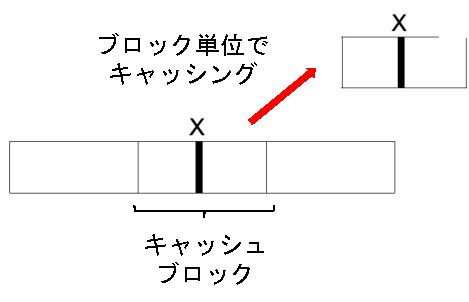
\includegraphics[width=\linewidth]{./figure/cache_block.pdf}
  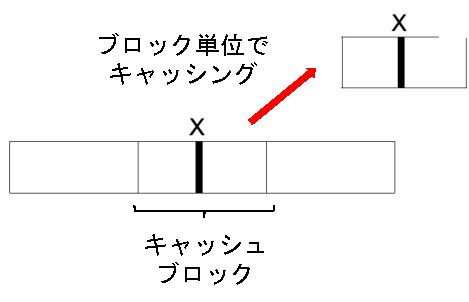
\includegraphics[scale=1.0]{./figure/cache_block.pdf}
  \caption{ブロック単位でのキャッシング}
  \label{cache_block}
\end{figure}
グラフ演算では演算過程において隣接ノードの値を参照とするという操作が繰り返されるため,ノード ID の配置方法によりキャッシュの使用効率も変化する.
そこで,グラフを取得しながらノード ID を再配置するにあたり,特に ID の連続性と演算時のアクセス局所性が重要となる.
\section{ID の連続性}
既存手法では,グラフの全体構造を把握した上で再配置を行うので,全ノードに連続した ID が再配置されることが保証される.
しかし,グラフを取得しながら ID を再配置する場合,再配置する ID が連続的かどうかを考慮する必要がある.
ID が連続するノードの値はメモリ上でも連続して格納されるが,ID の連続性が欠如していると,各ノードの値がメモリ上で点在する形となり,
全ノードを格納するためのキャッシュブロック数が増加してしまう.
キャッシュブロック数の増加に伴い,演算時にアクセス対象となるブロック数も増加し,
キャッシュブロックの書き換えが頻発してしまうためキャッシュミスが増加する.
例えば,図\ref{id_not_consecutive} で示すように,ノード ID が 2, 6, 10, 37, 53 と非連続的で,これら 5 ノードの値を格納するために
必要なブロック数が 3 だとする.
このグラフのノード ID を図\ref{id_consecutive} で示すように再配置する.
ID の連続性を実現した再配置により,同一の 5 ノードを格納するために必要なブロック数が 1 に減少している.
\begin{figure}[t]
  \begin{tabular}{cc}
    \begin{minipage}[t]{0.45\hsize}
      \centering
      %\includegraphics[keepaspectratio, scale=0.50]{./figure/id_not_consecutive.pdf}
      %\includegraphics[keepaspectratio, width=7cm]{./figure/id_not_consecutive.pdf}
      \includegraphics[width=7cm]{./figure/id_not_consecutive.pdf}
      %\includegraphics[scale=0.50]{./figure/id_not_consecutive.pdf}
      \caption{ID が非連続的な場合のブロック数}
      \label{id_not_consecutive}
    \end{minipage} &
    \begin{minipage}[t]{0.45\hsize}
      \centering
      %\includegraphics[keepaspectratio, scale=0.50]{./figure/id_consecutive.pdf}
      \includegraphics[width=7cm]{./figure/id_consecutive.pdf}
      %\includegraphics[scale=0.50]{./figure/id_consecutive.pdf}
      \caption{ID が連続的な場合のブロック数}
      \label{id_consecutive}
    \end{minipage}
  \end{tabular}
\end{figure}
\section{演算時のアクセス局所性}
グラフを取得しながら ID を再配置する場合でも,既存手法と同様に演算時のアクセス局所性を考慮する必要がある.
具体的には,演算時に局所的なアクセスが発生するノード群を同一キャッシュブロックに格納しておくことで,
キャッシュの使用効率が向上し,キャッシュミスが減少する.
アクセス局所性は次数による局所性と近接構造による局所性に分類できる.
\subsection{次数による局所性}
実世界グラフは次数分布が冪乗則に従うスケールフリー性と呼ばれる性質を持つ\cite{barabasi1999emergence,faloutsos1999power,clauset2009power}.
スケールフリー性を持つグラフでは,極めて少数のノードが高い次数を持つ一方で,大多数のノードは低い次数を持つ.
グラフ演算における各ノードへのアクセス頻度はそのノードの次数に比例するため,
少数の高次数ノードへアクセスが集中する.
このように,グラフがスケールフリー性を持つ状況では,次数が同程度のノードが同一キャッシュブロックに格納されるように ID を再配置することが有効である.

図\ref{bad_degree_cache} で示すように,同一キャッシュブロック内に次数が大きく異なるノードの値が格納されている場合,
低次数ノードの値は高次数ノードへのアクセスに伴って頻繁にキャッシングされる.
グラフ演算において低次数ノードへのアクセス数は極めて小さいため,
アクセスされにくい値の頻繁なキャッシングはキャッシュの使用効率低下を引き起こす.
一方,図\ref{good_degree_cache} で示すように,同一キャッシュブロック内に同程度の次数を持つノードの値が格納されている場合,
高次数ノードのアクセスに伴い低次数ノードの値がキャッシングされることを防止できる.
これにより,高次数ノードの値を格納しているブロックは演算終了時までキャッシュに格納され続け,
低次数ノードの値を格納しているブロックは必要最低限の回数だけキャッシングされるため,演算時のキャッシュミスが減少する.


\begin{figure}[t]
  \begin{tabular}{cc}
    \begin{minipage}[t]{0.45\hsize}
      \centering
      %\includegraphics[keepaspectratio, scale=0.50]{./figure/id_not_consecutive.pdf}
      %\includegraphics[keepaspectratio, width=7cm]{./figure/id_not_consecutive.pdf}
      \includegraphics[width=7cm]{./figure/bad_degree_cache.pdf}
      %\includegraphics[scale=0.50]{./figure/id_not_consecutive.pdf}
      \caption{ブロック内のノードの次数に差がある場合}
      \label{bad_degree_cache}
    \end{minipage} &
    \begin{minipage}[t]{0.45\hsize}
      \centering
      %\includegraphics[keepaspectratio, scale=0.50]{./figure/id_consecutive.pdf}
      \includegraphics[width=7cm]{./figure/good_degree_cache.pdf}
      %\includegraphics[scale=0.50]{./figure/id_consecutive.pdf}
      \caption{ブロック内のノードの次数が同程度の場合}
      \label{good_degree_cache}
    \end{minipage}
  \end{tabular}
\end{figure}

%なお,次数による局所性に着目した ID 再配置手法として \cite{zhang2017making,faldu2019closer}が提案されている.
\subsection{近接構造による局所性}
実世界グラフはスケールフリー性だけでなく,コミュニティ構造を保有するという特徴を持つ\cite{girvan2002community,leskovec2009community}.
コミュニティとは,グラフ上で密に接続しあっているノードの集合であり,同一コミュニティに所属するノードはグラフ上で極めて近接している.
%コミュニティ内のノード群は密に接続しあっており,グラフ上で極めて近接している.
一般に,グラフ演算では隣接ノードの値を参照するという操作が繰り返されるため,コミュニティ内のノード間で局所的なアクセスが発生する.
そのため,同一コミュニティに属する極めて近接したノード群の値が同一キャッシュブロックに格納されるように ID を再配置することが有効である.

例えば,図\ref{bad_community_cache}で示すように,ID V のノードに対し,その隣接ノードの ID が 2, 37, 53 と離れている場合,
ノード V の隣接ノードの値を参照するためには,3つのキャッシュブロックにアクセスする必要があるとする.
この場合,図\ref{good_community_cache}で示すように,隣接ノードが近い ID を持つように ID を再配置することで,
全隣接ノードが同一キャッシュブロックに格納され,演算時には1つのキャッシュブロックへアクセスするだけでノード V の全隣接ノードの値を参照することが可能となる.
このように,グラフ上で近接しているノードが同一キャッシュブロックへ格納されるように ID を再配置することで,演算全体を通してアクセスする
ブロック数が減少し,キャッシュミスが減少する.
\begin{figure}[t]
  \begin{tabular}{cc}
    \begin{minipage}[t]{0.45\hsize}
      \centering
      %\includegraphics[keepaspectratio, scale=0.50]{./figure/id_not_consecutive.pdf}
      %\includegraphics[keepaspectratio, width=7cm]{./figure/id_not_consecutive.pdf}
      \includegraphics[width=7cm]{./figure/bad_community_cache.pdf}
      %\includegraphics[scale=0.50]{./figure/id_not_consecutive.pdf}
      \caption{近接ノードの ID が離れている場合}
      \label{bad_community_cache}
    \end{minipage} &
    \begin{minipage}[t]{0.45\hsize}
      \centering
      %\includegraphics[keepaspectratio, scale=0.50]{./figure/id_consecutive.pdf}
      \includegraphics[width=7cm]{./figure/good_community_cache.pdf}
      %\includegraphics[scale=0.50]{./figure/id_consecutive.pdf}
      \caption{近接ノードの ID が近い場合}
      \label{good_community_cache}
    \end{minipage}
  \end{tabular}
\end{figure}

\section{自律分散グラフ管理環境での課題}
既存手法はグラフの全体構造を把握している前提で議論がされているため,再配置の対象となるノード数は既知である.
予めノード数が判明していることで ID の連続性が保証されているが,グラフ取得が完了するまで全グラフが手元にない状況では
既存手法と同様に ID の連続性を保証することは不可能である.
グラフ取得をしながら ID の連続性を保った再配置を実行するには,取得途中のグラフに対して連続的な ID を再配置し続ける必要がある.
しかし,取得途中のグラフ構造には次数による局所性や近接構造による局所性などの特徴が十分に反映されない可能性が高い.
例えば,取得初期の段階で高次数ノードと判定されたノードが取得完了時点では低次数ノードであると判明する可能性がある点や,
取得途中ではグラフ上の近接構造を正確に把握することが困難な点などが挙げられる.
ID の連続性のみを意識して再配置を行うと演算時のアクセス局所性が損なわれてしまうが,
アクセス局所性のみを意識するとグラフの取得完了を待つコストが増加してしまう.
このように,グラフ取得が完了するまで全グラフが手元にない状況では連続性とアクセス局所性の完全な両立は困難である.

\chapter{関連研究}
\label{chap:related_research}
\section{Gorder}
\cite{wei2016speedup}で提案
\section{HubSort}
\cite{zhang2017making}で提案
\section{HubClustering}
\cite{balaji2018graph}で提案
\section{Degree Based Grouping}
\cite{faldu2019closer}で提案

\section*{}
その他にも,Slash Burn \cite{kang2011beyond},Rabbit Order \cite{arai2016rabbit},ReCall \cite{lakhotia2017recall}などの Reordering 手法が提案されている.

\chapter{自律分散グラフ管理環境における Reordering}
\label{chap:design}
\section{Sequential}
\section{Dynamic Degree Based Grouping (DDBG)}

\begin{comment}
\chapter{プロトコル詳細}
\label{chap:protocol}
\input{05-protocol}
\end{comment}

\begin{comment}
\chapter{実装}
\label{chap:implementation}
\section{概要}
言語は C++17 を用いた.ここでは主に以下の 3 点について述べる.
\begin{itemize}
  \item グラフ取得の基本的な実装
  \item Sequential における再配置の実装
  \item DBG-EE における再配置の実装 
\end{itemize}
\section{グラフ取得の基本的な実装}
\subsection{グラフ構造を保持するためのデータ構造}
\label{graph_data}
まず,取得したグラフを保持するためのデータ構造について述べる.
本手法では隣接リストによるグラフ表現として,始点ノードの ID をキー,終点ノードの集合をペアとするハッシュ連想配列を採用している.
%実際に使用したデータ構造をソースコード \ref{data_structure} に示す.
\begin{lstlisting}[caption=グラフ構造, label=data_structure]
  typedef unordered_map<unsigned int, vector<unsigned int>> Graph; 
\end{lstlisting}

\subsection{RW によるグラフ取得}
\ref{graph_data} 小節で述べたデータ構造を用いて,RW によるグラフ取得を行う.
RW 中は滞在ノードにおいて 0 以上 1 以下の乱数値を発生させ,乱数値が確率 α を下回った場合は始点へ移動する.
また,α を下回らない場合でも,滞在ノードの出次数が 0 の場合は始点へ移動する.
乱数値が α を下回らず,滞在ノードの出自数が 1 以上の場合は,
滞在ノードの隣接ノード群からランダムに 1 ノードを選択し,そのノードへ移動する.
このような移動を繰り返す中で,滞在ノードと移動先ノードの間にエッジが存在するかを毎回確認する.
そして,エッジが存在していない場合は取得グラフに新たなエッジとして追加する.
\begin{lstlisting}[caption=RW によるグラフ取得, label=rw_graph_get]
  // All_Graph : データセットを保持するグラフ
  // Get_Graph : RW により取得したグラフ
  Graph Get_Graph, All_Graph;

  // 0 以上 1 以下の乱数生成 
  random_device seed_gen;
  mt19937 engine(seed_gen());
  uniform_real_distribution<> dist(0,1.0);
  // src : 始点ノード,dst : 終点ノード
  unsigned int RW_num, RW_count, src, dst;
  // RW の始点
  unsigned int start_node;
  // RW で始点に戻る確率
  float return_prob;

  while (RW_count < RW_num) {
    if (dist(engine) < return_prob) {
      src = start_node;
      RW_count++;
      continue;
    } else {
      // src から進めない場合,始点へ戻る
      if (All_Graph[src].size() == 0) {
        src = start_node;
        RW_count++;
        continue;
      } else {
        // 移動先として隣接ノード群からランダムに1ノード選択
        dst = (All_Graph[src]).at(engine() % All_Graph[src].size());
        // src -> dst にエッジが存在しない場合,Get_Graph へ登録
        if (find(Get_Graph[src].begin(), Get_Graph[src].end(), dst) == Get_Graph[dst].end()) {
        }
        src = dst;
      }
    }
  }
\end{lstlisting}
\section{Sequential における再配置の実装}
Sequential では RW の途中で出会ったノード順に昇順の連続した ID を再配置する.
再配置が行われた場合,マッピングテーブルに ID の対応関係が登録される.
ここで,マッピングテーブルの実装として,元の ID をキー,新たな ID をペアとするハッシュ連想配列を採用している.
\begin{lstlisting}[caption=マッピングテーブル, label=mapping_table]
  typedef unordered_map<unsigned int, unsigned int> Mapping;
\end{lstlisting}

実際の処理では,RW で 1 エッジ移動する度にマッピングテーブルの参照・登録を行うことで,ID が再配置された形でグラフ構造を保持する.
ソースコード \ref{sequential_code} に Sequential における再配置の実装を示す.
この処理はソースコード \ref{rw_graph_get} における 30 - 32行目で実行される. 
\begin{lstlisting}[caption=Sequential における再配置, label=sequential_code]
  // 次の移動先ノードが再配置済みか確認 
  if (Sequential_Mapping.count(dst) == 0) {
    Sequential_Mapping[dst] = Sequential_Mapping.size();
  }
  // 再配置された ID でグラフ構造を保持
  mapped_src = Sequential_Mapping[src];
  mapped_dst = Sequential_Mapping[dst];
  if (find(Mapped_Graph[mapped_src].begin(), Mapped_Graph[mapped_src].end(), mapped_dst) == Mapped_Graph[mapped_src].end()) {
    Mapped_Graph[mapped_src].push_back(mapped_dst);
  }
\end{lstlisting}
\section{DBG-EE における再配置の実装}
\subsection{グループサイズの早期推定}
DBG-EE ではグラフ取得初期の段階でグループサイズの推定を行う.
\begin{lstlisting}
  void Initiate_Group(Graph & Partial_Graph, Group & DDBG_Group, int remain)
  {
    vector<unsigned int> group_size(8,0);
    int deg;
    for (auto & [src, dsts] : Partial_Graph) {
      deg = dsts.size();
      if (deg > 32 * ave_deg) {
        group_size.at(0)++;
      } else if (deg > 16 * ave_deg && deg < 32 * ave_deg) {
        group_size.at(1)++;
      } else if (deg > 8 * ave_deg && deg < 16 * ave_deg) {
        group_size.at(2)++;
      } else if (deg > 4 * ave_deg && deg < 8 * ave_deg) {
        group_size.at(3)++;
      } else if (deg > 2 * ave_deg && deg < 4 * ave_deg) {
        group_size.at(4)++;
      } else if (deg > 1 * ave_deg && deg < 2 * ave_deg) {
        group_size.at(5)++;
      } else if (deg > 0.5 * ave_deg && deg < 1 * ave_deg) {
        group_size.at(6)++;
      } else {
        group_size.at(7)++;
      }
    }
    unsigned int start = 0; 
    unsigned int width;
    for (int i = 0; i < DDBG_Group.size(); i++) {
      width = group_size.at(i) * remain;
      DDBG_Group.at(i).first = start;
      DDBG_Group.at(i).second = start + width;
      start += width + 1;
    }
  }
\end{lstlisting}

\begin{comment}
\begin{lstlisting}
void DBGEE(Graph & Partial_Graph, Graph & Mapped_Graph, Group & DBGEE_Group, Mapping & DBGEE_Mapping)
{
  unsigned int edge_num = 0;
  for (auto & [src, dsts] : Partial_Graph){
    edge_num += dsts.size();
  }
  float ave_deg = static_cast<float>(edge_num)/Partial_Graph.size();

  vector<unsigned int> v_sorted;
  for (auto & [src, dsts] : Partial_Graph){
    v_sorted.push_back(src);
  }
  sort(v_sorted.begin(), v_sorted.end());

  unsigned int mapped_src, mapped_dst;
  for (auto [src, dsts] : Partial_Graph) {
    if (DDBG_Mapping.count(src) == 0) {
      Mapping_id(DDBG_Mapping, DDBG_Group, src, dsts.size(), ave_de
g);
].size(), counter, ave_deg);
    }
    mapped_src = DDBG_Mapping[src];
    for (auto & dst : dsts) {
      if (DDBG_Mapping.count(dst) == 0) {
        Mapping_id(DDBG_Mapping, DDBG_Group, dst, Partial_Graph[dst
].size(), ave_deg);
st].size(), counter, ave_deg);
      }
      mapped_dst = DDBG_Mapping[dst];
      if (find(Mapped_Graph[mapped_src].begin(), Mapped_Graph[mappe
d_src].end(), mapped_dst) == Mapped_Graph[mapped_src].end()) {
        Mapped_Graph[mapped_src].push_back(mapped_dst);
      }
    }
  }
  Partial_Graph.clear();
}
\end{lstlisting}
\end{comment}

\begin{lstlisting}
void Mapping_id(Mapping & DDBG_Mapping, Group & DDBG_Group, unsigne
d int original_id, int deg, float ave_deg)
{
  if (deg > 32 * ave_deg) {
    DDBG_Mapping[original_id] = DDBG_Group.at(0).first++;
  } else if (deg > 16 * ave_deg && deg < 32 * ave_deg) {
    DDBG_Mapping[original_id] = DDBG_Group.at(1).first++;
  } else if (deg > 8 * ave_deg && deg < 16 * ave_deg) {
    DDBG_Mapping[original_id] = DDBG_Group.at(2).first++;
  } else if (deg > 4 * ave_deg && deg < 8 * ave_deg) {
    DDBG_Mapping[original_id] = DDBG_Group.at(3).first++;
  } else if (deg > 2 * ave_deg && deg < 4 * ave_deg) {
    DDBG_Mapping[original_id] = DDBG_Group.at(4).first++;
  } else if (deg > 1 * ave_deg && deg < 2 * ave_deg) {
    DDBG_Mapping[original_id] = DDBG_Group.at(5).first++;
  } else if (deg > 0.5 * ave_deg && deg < 1 * ave_deg) {
    DDBG_Mapping[original_id] = DDBG_Group.at(6).first++;
  } else {
    DDBG_Mapping[original_id] = DDBG_Group.at(7).first++;
  }
}
\end{lstlisting}
\end{comment}

\chapter{評価}
\label{chap:evaluation}
\section{実験の目的}
本研究では,RW によるグラフ取得をしながらノード ID を再配置する手法として,Sequential と DBG-EE を提案した.
そこで,実世界グラフのデータセットに対して Sequential 及び DBG-EE を適用した場合の効果を実験から明らかにする.
具体的には,グラフ取得の完了を待たないことによる空間・時間コストの変化及びグラフ演算時間の減少率に着目する.
\section{実験概要}
\subsection{データセット}
実世界グラフのデータセットとして,スタンフォード大学が提供するグラフデータセットライブラリ SNAP \cite{snapnets} 内の 
Pokec Social Network \cite{takac2012data} を使用した.
表 \ref{dataset} に Pokec Social Network のグラフ情報を示す.
90 \% 有効直径とはノード間の最短距離の分布において 90 パーセンタイルに相当する値であり,
任意のノード間で最短距離が 5.2 以下となる確率が 90 \% であることを意味している.
\begin{table}[t]
  \begin{center}
    \caption{Pokec Social Network の概要}
    \begin{tabular}{cc} \toprule
      ノード数 & 1,632,803 \\
      エッジ数 & 30,622,564 \\
      90 \% 有効直径 & 5.2 \\ \bottomrule
    \end{tabular}
    \label{dataset}
  \end{center}
\end{table}

\subsection{パラメータの決定方法}
まず,RW 回数 N の決定方法について述べる.
表 \ref{rw_graph} で示すように,全体グラフのエッジ数に対する取得グラフのエッジ数は N = 100 万 のとき約 5 \%, N = 300 万 のとき約 10 \% となることが
実験的に明らかになった.
5 \% - 10 \% 程度のエッジを取得するという状況は全体グラフの一部を取得するという前提に矛盾しないと
判断し,N = 100 万,300 万をパラメータとして採用した.

次に,始点へ戻る確率 α の決定方法について述べる.
一般に,RW において始点に戻るまでの平均経路長は 1/α であることが知られている.
この平均経路長を 90 \% 有効直径と同程度に設定することで,始点の周辺グラフだけを密に取得し,
全体グラフの構造が失われる状況を回避できる.
表 \ref{dataset} で示すように,Pokec Social Network の 90 \% 有効直径は約 5 なので,α = 0.2 を
採用することで平均経路長と 90 \% 有効直径を同程度に設定した. 

表 \ref{parameter} に全パラメータの値を示す.
M は DBG-EE における再配置実行間隔に対応している.
なお,RW の開始点としてグラフ上の最高次数ノードを採用した.
\begin{table}[t]
  \begin{center}
    \caption{RW 回数と取得したエッジ数の割合の関係}
    \begin{tabular}{cccc} \toprule
      RW 回数 & ノード数 & エッジ数 & 取得したエッジ数の割合 \\ \hline
      100 万回 & 435,934 & 1,411,607 & 4.61 \% \\
      300 万回 & 686,506 & 3,409,700 & 11.3 \% \\ \bottomrule
    \end{tabular}
    \label{rw_graph}
  \end{center}
\end{table}
\begin{table}[t]
  \begin{center}
    \caption{各パラメータの値}
    \begin{tabular}{cc} \toprule
      N & 100 万, 300 万 \\
      M & 1 万,10 万 \\
      α & 0.2 \\ \bottomrule
    \end{tabular}
    \label{parameter}
  \end{center}
\end{table}


\subsection{対象とするグラフ演算}
RW で取得したグラフに対して PageRank (PR) と Personalized PageRank (PPR) を実行した.
なお,PR の計算には Ligra \cite{shun2013ligra} を,PPR の計算には FORA \cite{wang2017fora} を使用した.

\section{評価概要}
評価項目は以下の 3 点である.
\begin{itemize}
  \item ID 再配置を実行するためのメモリ使用量
  \item グラフ取得開始から演算終了までの合計時間 
  \item グラフ演算のみに要する時間
\end{itemize}
提案手法である Sequential,DBG-EE の比較対象は ID 再配置を実行しない Original,既存手法の DBG である.
なお,評価環境は表 \ref{eval_env} に示す通りである.
\begin{table}[t]
  \begin{center}
    \caption{評価環境}
    \begin{tabular}{cc} \toprule
      実装言語 & C++ \\
      OS & Ubuntu Server 16.04 LTS \\
      CPU & Intel(R) Xeon(R) E5-2680 v3 @ 2.50 GHz \\
      RAM & 32 GB \\
      L1 キャッシュ & 32 KB  \\
      L2 キャッシュ & 256 KB \\
      L3 キャッシュ & 32 MB \\ \bottomrule 
    \end{tabular}
    \label{eval_env}
  \end{center}
\end{table}

\section{ID 再配置を実行するためのメモリ使用量}
ID 再配置を実行するためのメモリ使用量を DBG に対する割合として測定した.
N = 100 万の結果を図 \ref{memory_usage_1000000} に,
N = 300 万の結果を図 \ref{memory_usage_3000000} に示す. 
Sequential は N = 100 万で 40.0 \% 減少,N = 300 万で 41.9 \% 減少と両方の場合でメモリ使用量の減少率が最大となった.
DBG-EE では M = 10,000 の場合 N = 100 万で 29.5 \% 減少,N = 300 万で 35.4 \% 減少した.
一方,M = 100,000 の場合 N = 100 万で 16.5 \% 減少,N = 300 万で 26.8 \% 減少と M = 10,000 の場合より減少率が低下した.
これは,M の値が大きいほど取得途中で保持しなければならないグラフ構造が巨大化するからである.
また,N = 100 万より N = 300 万の方が減少率が大きいことから,
取得するグラフのサイズが大きいほど Sequential, DBG-EE の効果が大きいことが確認できる.
\begin{figure}[t]
  \centering
  \includegraphics[width=0.8\linewidth]{./figure/memory_usage_10000.pdf}
  \caption{N = 100 万の場合における DBG に対するメモリ使用量}
  \label{memory_usage_1000000}
\end{figure}

\begin{figure}[t]
  \centering
  \includegraphics[width=0.8\linewidth]{./figure/memory_usage_3000000.pdf}
  \caption{N = 300 万の場合における DBG に対するメモリ使用量}
  \label{memory_usage_3000000}
\end{figure}

\section{グラフ取得開始から演算終了までの合計時間}
次に,グラフ取得を開始してから PR 演算が終了するまでの合計時間を計測した.
N = 100 万の結果を図 \ref{total_time_1000000} に,
N = 300 万の結果を図 \ref{total_time_3000000} に示す.
まず,図\ref{total_time_1000000} では,M = 10,000 の場合の DBG-EE,M = 100,000 の場合の DBG-EE,Sequential 全てが DBG の合計時間を
下回っている.
この結果は,グラフの取得完了を待たないことで時間コストが削減できていることを示しており,Sequential,DBG-EE の有用性が確認できる.
最も時間コストが削減されたのは M = 100,000 の場合の DBG-EE で DBG と比べて合計時間が 11 \% 短縮している.
図 \ref{total_time_3000000} では,DBG-EEが M = 10,000 の場合,M = 100,000 の場合のどちらもで DBG の合計時間を下回っているが,
Sequential では合計時間が DBG より 1.5 \% 増加している. 

Sequential で合計時間が増加した要因として 2 点考えられる.
まず 1 点目として DBG や DBG-EE と比べてグラフ演算に要する時間が長い点である.これは\ref{algo_time} で詳しく述べる.
2 点目として RW によるグラフ取得の時間コストが大きい点である.
図\ref{sequential} で示すように,Sequential は RW で 1 ノード移動する度に移動先のノードが再配置済みかを確認する.
この確認に伴い発生する時間コストが図\ref{total_time_3000000} における Original の RW 時間と Sequential の RW 時間の差に現れている.
DBG は取得完了後の再配置に伴い時間コストが発生するが,RW によるグラフ取得自体にかかる時間コストは Original と等しい.
そのため,Sequential で再配置に伴う時間コスト減少の効果が弱まり,結果として DBG より合計時間が増加している.
\begin{figure}[t]
  \centering
  \includegraphics[width=0.8\linewidth]{./figure/total_time_1000000.pdf}
  \caption{N = 100 万の場合におけるグラフ取得と演算の合計時間}
  \label{total_time_1000000}
\end{figure}
\begin{figure}[t]
  \centering
  \includegraphics[width=0.8\linewidth]{./figure/total_time_3000000.pdf}
  \caption{N = 300 万の場合におけるグラフ取得と演算の合計時間}
  \label{total_time_3000000}
\end{figure}

\section{演算のみに要する時間}
最後に,グラフ演算のみに要する時間を測定した.
なお,グラフ演算として PR と PPR を実行した.
\label{algo_time}
\begin{figure}[t]
  \centering
  \includegraphics[width=0.8\linewidth]{./figure/algo_time_1000000.pdf}
  \caption{N = 100 万の場合における PR, PPR 演算時間}
  \label{algo_time_1000000}
\end{figure}
\begin{figure}[t]
  \centering
  \includegraphics[width=0.8\linewidth]{./figure/algo_time_3000000.pdf}
  \caption{N = 300 万の場合における PR, PPR 演算時間}
  \label{algo_time_3000000}
\end{figure}

\chapter{結論}
\label{chap:conclusion}
\section{まとめ}
本研究では,空間・時間コスト削減のためにランダムウォーク(RW) によるグラフ取得をしながらノード ID を再配置する手法として,
ID の連続性を意識した Sequential と 演算時のアクセス局所性を意識した DBG-EE の 2 手法を提案した.

Sequential は RW によるグラフ取得の途中で出会ったノード順に連続した昇順の ID を再配置することで ID の連続性を保証する.
また,取得途中では RW で移動した 1 エッジの構造のみ保持することで空間コストを削減している.
また,RW による移動の仕方によって隣接ノードへ連続した ID の再配置が可能となり,近接構造によるアクセス局性が部分的に考慮されている.

DBG-EE は既存の再配置手法で次数情報のみを必要とする DBG をもとに,RW によるグラフ取得の途中でノードを次数でグループ分けし,グループ毎に ID の再配置を行う.
DBG-EE は,取得初期の段階で各グループサイズの推定を行い,グループ毎に再配置で使用する ID の範囲を決定する.
また,再配置が終了した時点で取得したグラフ構造を破棄することで空間コストを削減している.
さらに,グラフ取得と ID 再配置を並列して実行することでグラフ取得を待つだけの時間を無くし,時間コストを削減している.

そして,実世界グラフのデータセットを用いて Sequential と DBG-EE の効果をグラフ取得の完了を待たないことによる空間・時間コストの変化及びグラフ演算時間の減少率から明らかにした.
まず,DBG と比べて ID 再配置を実行するために必要なメモリ使用量は Sequential,DBG-EE ともに減少し,Sequential で最大 41.9 \% 減少した.
次に,グラフ取得開始から演算終了までの合計時間では RW 100 万回,300 万回と両方の場合で DBG-EE が DBG を下回った.
しかし,Sequential では RW 300 万回の場合で DBG より 1.1 \% 合計時間が増加した.
さらに,再配置を実行しない場合と比べて PR 演算に要する時間の減少率は DBG-EE の方が大きく,最大で 46.8 \% 減少した.
一方で PPR 演算に要する時間の減少率は Sequential の方が大きく,最大で 40.6 \% 減少した.

\section{今後の展望}
Sequential,DBG-EE ともに空間コストの大きな削減は達成したが,グラフ取得から演算終了までを合計した時間コストの大きな削減は達成できていない.
時間コストに着目したとき,RW によるグラフ取得にかかる時間を一定の制限時間とみなし,この制限時間内に最も演算時間が減少する再配置を実行する手法が望ましい.
本研究では,前処理コストの小さい DBG に着目したが,制限時間までの時間コストが許容される場合,
Gorder のような前処理コストが大きいが演算時間が大きく減少する手法に着目することが可能だと考える.

さらに,本研究では ID の連続性と 演算時のアクセス局所性にそれぞれ着目した手法を提案したが
既存手法のように ID の連続性とアクセス局所性の双方を考慮した ID 再配置が実行できれば,DBG-EE,Sequential の性能を上回ることが可能だと考える.
そこで,\ref{algo_time} 節で述べたように,対象とするアルゴリズム毎にどのようなアクセス局所性を考慮すべきか明らかにすることで,
Sequential のように ID の連続性を保証しながら,対象とするアルゴリズムに応じたアクセス局所性を最大限考慮した ID の再配置が行えると考える.

\label{chap:thanks}
\chapter*{謝辞}
{\small
\begin{flushright}
平成 30 年 1 月 30 日
\end{flushright}
}
\addcontentsline{toc}{chapter}{謝辞}

%%%%%    参考文献    %%%%%
\typeout{References}
\thispagestyle{plain}
\bibliographystyle{unsrt}
\bibliography{b-thesis}

\appendix
\def\thechapter{付録\Alph{chapter}}
\chapter{スクリプト}
\label{chap:appendix}
\def\thechapter{\Alph{chapter}}
\typeout{付録}
\input{appendix}
\end{document}
